% flashcards-title: Signed area on a velocity-time graph
% flashcards-desc: Velocity is positive at two metres per second for two seconds, then negative at one metre per second for three seconds; the regions use solid and dashed outlines.
\documentclass[border=7pt]{standalone}
\def\pgfsysdriver{pgfsys-dvisvgm.def}
\usepackage{tikz}
\usetikzlibrary{arrows.meta,positioning,shapes.geometric}
\definecolor{mechInk}{HTML}{172033}
\definecolor{mechBlue}{HTML}{155EEF}
\definecolor{mechOrange}{HTML}{B54708}
\definecolor{mechPale}{HTML}{E8F0FF}
\definecolor{mechGray}{HTML}{667085}
\definecolor{mechLight}{HTML}{D0D5DD}
\tikzset{
  every picture/.style={font=\sffamily\large, text=mechInk},
  mech box/.style={draw=mechInk, line width=1.2pt, rounded corners=4pt,
    fill=white, align=center, minimum height=14mm, inner xsep=5mm},
  mech primary/.style={draw=mechBlue, line width=2.2pt},
  mech secondary/.style={draw=mechOrange, line width=2.2pt, dashed},
  mech guide/.style={draw=mechGray, line width=0.9pt, dashed},
  mech arrow/.style={-{Stealth[length=3.2mm,width=2.4mm]},
    draw=mechInk, line width=1.4pt, line cap=butt},
  mech axis/.style={draw=mechInk, line width=1.2pt},
  mech tick/.style={draw=mechInk, line width=1pt}
}

\begin{document}
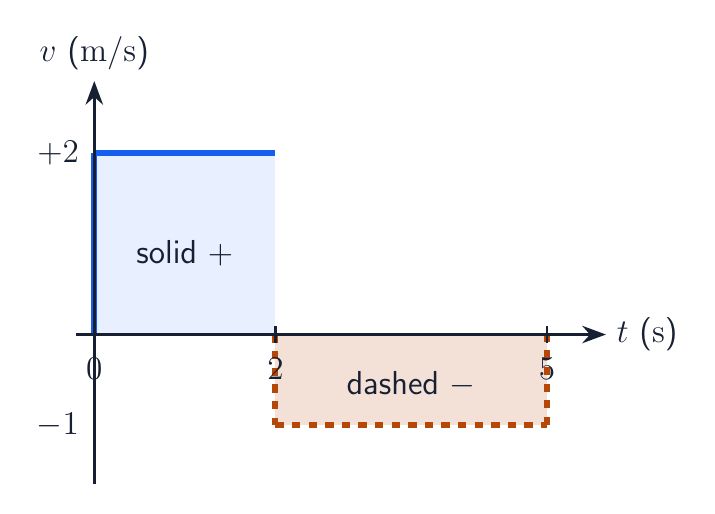
\begin{tikzpicture}[x=1.15cm,y=1.15cm]
  \fill[mechPale] (0,0) rectangle (2,2);
  \fill[mechOrange,opacity=0.16] (2,0) rectangle (5,-1);
  \draw[mech primary] (0,2) -- (2,2);
  \draw[mech primary] (0,0) -- (0,2);
  \draw[mech secondary] (2,-1) -- (5,-1);
  \draw[mech secondary] (2,0) -- (2,-1);
  \draw[mech secondary] (5,-1) -- (5,0);
  \draw[mech axis,-{Stealth[length=3mm,width=2.2mm]}] (0,-1.65) -- (0,2.8) node[above] {\(v\) (\(\mathrm{m/s}\))};
  \draw[mech axis,-{Stealth[length=3mm,width=2.2mm]}] (-0.2,0) -- (5.65,0) node[right] {\(t\) (\(\mathrm{s}\))};
  \foreach \x in {0,2,5} {
    \draw[mech tick] (\x,-0.09) -- (\x,0.09);
    \node[below=2pt] at (\x,-0.09) {\(\x\)};
  }
  \node[left=2pt] at (0,2) {\(+2\)};
  \node[left=2pt] at (0,-1) {\(-1\)};
  \node at (1,0.9) {solid \(+\)};
  \node at (3.5,-0.55) {dashed \(-\)};
\end{tikzpicture}
\end{document}
